\chapter{Vision System Project}
\label{cha:vision-system-project}

Deep learning methods has reached in the recent years state-of-the-art results in many applications, e.g. image recognition, speech recognition and synthesis, natural language processing and reinforcement learning. Having in mind the results described in \ref{sub:intro-games} and the outstanding performance of the application of DQN in teaching Autonomous Driving Agent \cite{2020DuckieTown} it appeared that Autonomous Floating Agent (Boat) would be a natural step. The idea was to create a vision system using CNN (\ref{cha:conv}) + RNN (\ref{cha:reinforcement-learning}) + DNN (\ref{cha:dl}) which would be capable of routing the boat between buoys in the simple environment. Due to time and hardware limitations it was impossible test it in the real world. However, the results are promising enough to suppose that with further development it would be possible to use proposed vision system on a physical boat.

\section{Simulation Environment}
\label{sec:simulation-env}

Before any algorithm begins to train an autonomous agent a virtual reality must be created. Virtual for us of course, for the agent it is the only world that is known. The purpose was to find simple enough environment to minimise external factors which could affect the vision system performance and simultaneously complex enough to benchmark it. Additionally, simulation had to be compatible with \textbf{Robot Operating System (ROS)} and \textbf{OpenAI Gym} used to train proposed DQN. 

\subsection{Gazebo}
\label{sub:gazebo}

The simulation environment chosen for the project was \emph{Gazebo 11}\footnote{\url{https://gazebosim.org/}} - an open source robot 3D simulator.
It is used for designing robots, offering ROS integration, performing regression testing with realistic scenarios and what is most important testing robotics algorithms. Needless to say, it perfectly satisfies project's prerequisites. Since the main purpose of the Thesis was the vision system, not the simulation environment itself, there has been chosen a \textbf{Virtual RobotX} \cite{bingham19toward} project as a starting point. It is an simulation environment, designed in coordination with RobotX\footnote{\url{https://defenceinnovationnetwork.com/robotx-challenge-2022/}} challenge organizers - the international, university-level maritime autonomous robotic systems competition. However, it required several modifications.

First of all, the environment must have followed simplicity principle, hence the \emph{Sydney regatta} map was used. All obstacles were replaced with buoys which created a route for the boat, as in the following image. 

\begin{figure}[h]
    \centering
    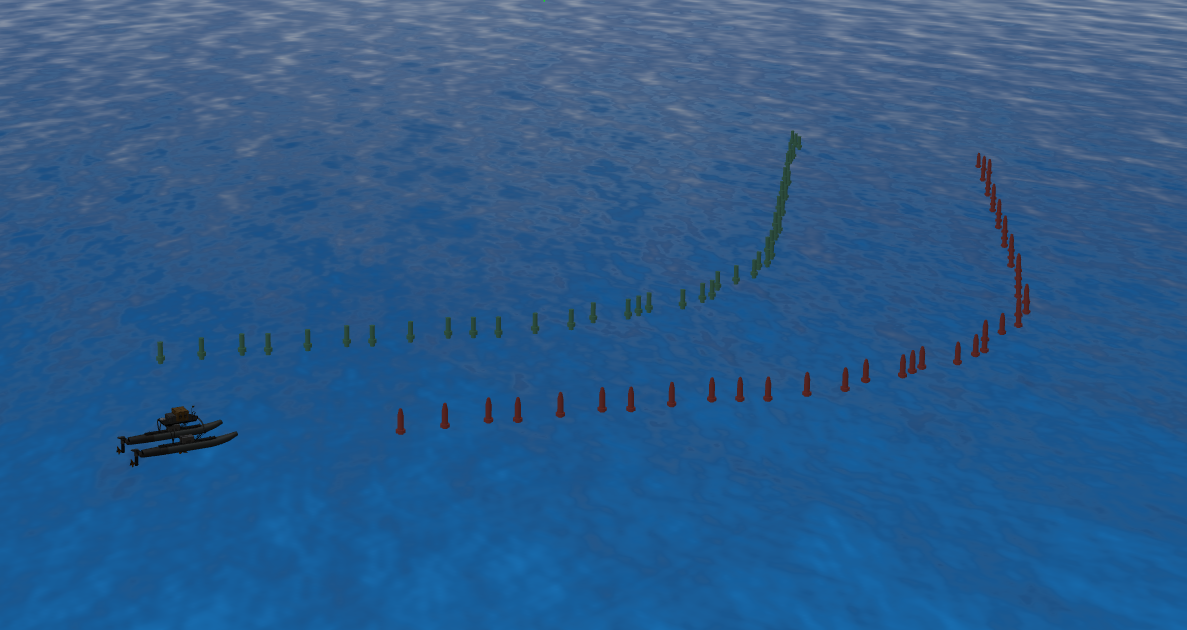
\includegraphics[width=16cm]{img/simulation_view.png}
    \caption{Sydney regatta map with prepared track}
    \label{fig:sydney-regatta-map}
\end{figure}

The buoys create a curve to force an autonomous agent to adjust to changeable conditions. If the track was straight, the environment would present significantly less challenge for the Deep Reinforcement Network. It could possibly neglect all the propellers speed except the "float forward" instruction regardless of what images are perceived by cameras. What is more, left-side buoys are green coloured and of slightly different shape than right-side coloured red. This makes it easier for the CNN to recognize correct patterns and subsequently increases the entire vision system performance.

\subsubsection*{Sensors}
\label{sub2:sensors}

The boat running on the ROS is equipped with multiple sensors, but for the purpose of reinforcement learning the following were used:
\begin{itemize}
    \item Front right camera,
    \item front left camera,
    \item odometry.
\end{itemize}

Whereas first two are self-explanatory, odometry is the use of motion sensors to determine the robot's change in the position relative to
some known position. In other words, it allows to retrieve $(x, y, z)$ coordinates of the boat. This in turn allows to control whether
the boat is within the track or if it reached the desired position.

\begin{figure}[h]
    \centering
    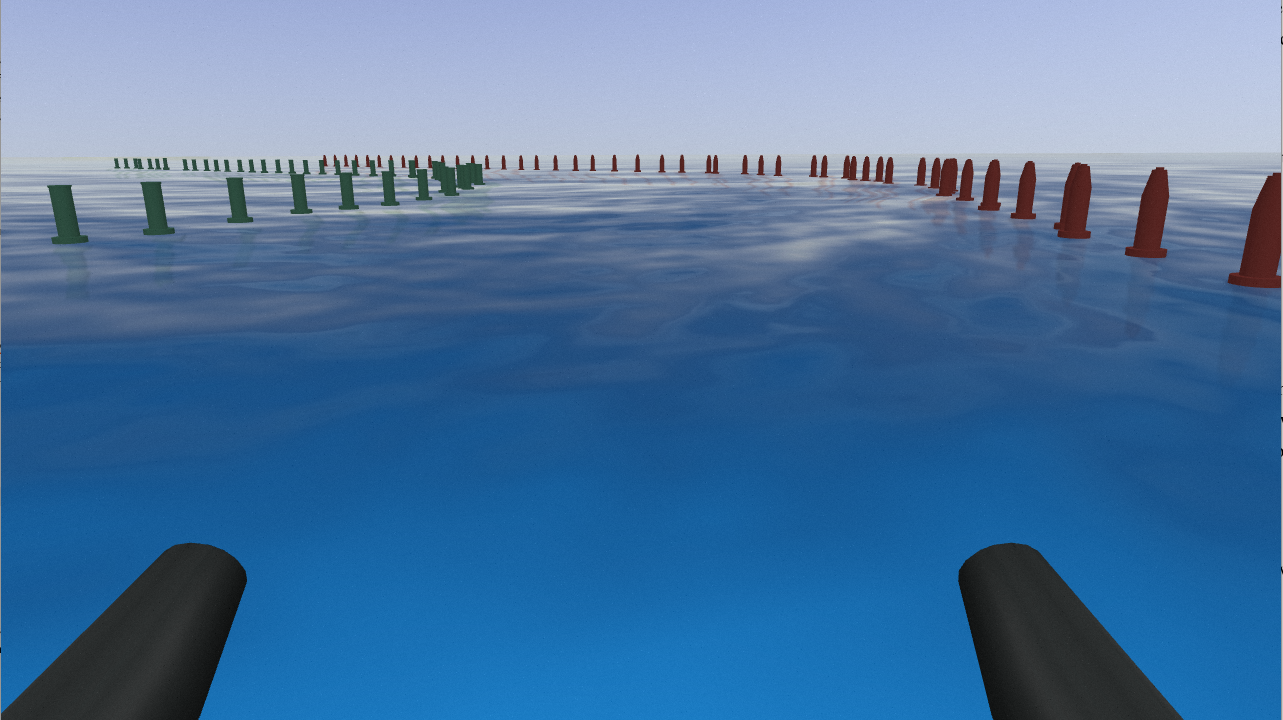
\includegraphics[width=16cm]{img/front_camera_image.png}
    \caption{View from boat's camera}
    \label{fig:camera-view}
\end{figure}

\subsection{OpenAI Gym}
\label{sub:openai-gym}

OpenAI Gym\footnote{\url{https://gym.openai.com/}} is a toolkit for developing and comparing reinforcement learning algorithms. It supports multiple environments, from walking agent to playing games like \emph{Pong} or \emph{Pinball}. Running simulation with gym is straightforward. At every step an agent chooses an action, then takes a step in the environment. In return observation is received for the state $s'$, reward $R_a(s, s')$ and \emph{done} flag, which is a boolean value.

\begin{lstlisting}[language=Python, caption={Example gym environment simulation}]
1  env = gym.make('My-env')
2  observaton = env.reset()
3  for _ in range(steps):
4      action = agent.chose_action()
5      observation, reward, done = env.step(action)
6      if done:
7          observation = env.reset()
8  env.close()
\end{lstlisting}

For our use case the custom environment was created using Gazebo and ROS. The python script communicates with boat robot through ROS topics which then performs an action and sends back the new observation through another ROS topic. The reward is computed after each step based on odometry which is also responsible for controlling agent's position.

\begin{table}[h]
    \centering
    \begin{tabular}{||c c c c||}
        \hline
        Topic & ROS Boat &  OpenAI Env & Description \\
        \hline\hline
        left\_thrust\_cmd & S & P & Left thrust \\
        right\_thrust\_cmd & S & P & Right trust \\
        front\_right\_camera & P & S & Right camera image \\
        front\_left\_camera & P & S & Left camera image \\
        odom & P & S & Odometry \\
        \hline
    \end{tabular}
    \caption{List of ROS topics used in custom OpenAI environment.\newline P - publisher, S - subscriber}
    \label{tab:ros-topics}
\end{table}

\subsubsection*{State space}
\label{sub2:state-space}

Despite the boat being placed in a relatively spacious map, its \textbf{state space} was limited to rectangle of shape $\left( (x_{max} - x_{min}) \times (y_{max} - y_{min})\right)$. Furthermore, the boat can only move between left and right buoys of the same pair, which have positions $(x^i_l, y^i_l)$ and $(x^i_r, y^i_r)$ where $i$ is the buoy pair's index, similarly to layer numbering in ANN. Note that $x^i_l = x^i_r = x^i$, because the directions are aligned with coordinate system. When the agent passes pair of buoys

\begin{equation}
    x^i - \psi \leq x_{agent} \leq x^i + \psi
\label{eq:5.1}
\end{equation}

the constraints must be followed,

\begin{equation}
    y^i_l + \psi \leq y_{agent} \leq y^i_r + \psi
\label{eq:5.2}
\end{equation}

where $\psi$ is an offset. Otherwise the boat is considered off-track, which is an illegal space, and \emph{done} flag is set \emph{true}. After the boat passed pair of corresponding buoys, also called a \emph{checkpoint}, it cannot move backwards any further than $x^i - 3$ or the episode is terminated (done). This constraint gives an direction for the agent to follow. Additionally, maximum distance from desired point has been introduced, which cannot be greater than the largest distance of a state space. The distance is calculated as simple \emph{euclidean distance}

\begin{equation}
    d = \sqrt{(x_1 - x_2)^2 + (y_1-y_2)^2}
\end{equation}

The goal of the simulation is to reach the desired point. If $(x_{agent}, y_{agent}) = (x_{desired}, y_{desired})$ then simulation episode finishes and \emph{done} is set \emph{true}. 

\subsubsection*{Action Space}
\label{sub2:action-space}

The boat can take one of eight discrete actions, which are predicted by DQN algorithm.

\vspace{.5cm}

\begin{table}[h]
\centering
\begin{tabular}{||l c c ||}
    \hline
     Action & Left Propeller Speed & Right Propeller Speed \\
     \hline\hline
     0 (Forward) & 1 & 1 \\
     1 (Backward) & -1 & -1 \\
     2 (Left) & 1 & -1 \\
     3 (Right) & -1 & 1 \\
     4 (0.5 Right) & -0.5 & 0.5 \\
     5 (0.5 Left) & 0.5 & -0.5 \\
     6 (0.3 Right) & -0.3 & 0.3 \\
     7 (0.3 Left) & 0.3 & -0.3 \\
    \hline
\end{tabular}
\caption{Discrete actions predicted by the DQN algorithm}
\label{tab:action-space}
\end{table}

\subsubsection*{Observation Space}
\label{sub2:observation-space}

Usually the observation space $O$ is just a part of the entire state space $S$. However in this particular use case the information about the relative $(x, y, z)$ location was replaced by images from cameras. The agent does not have an access to odometry information. The only way to perceive the environment is through its vision system.

The raw 1280x720 images are preprocessed before feeding the neural network. This step is crucial in achieving close to optimal performance, because only particular features on image are useful. In this particular case buoys are what matters. Neither the beautiful blue sky nor eye-catching azure water bring any viable information for keeping the boat inside the track. Therefore the following steps are performed:

\begin{enumerate}
    \item \textbf{Cropping}
    
    The bottom 240 pixels are removed, since they contain only redundant water and front of the boat. To get wider picture refer to fig. \ref{fig:camera-view}.
    
    \item \textbf{Concatenation}
    
    Left half of the left's camera image is concatenated with right half of the right's camera image along vertical axis. Resulting image has the same resolution as original one.
    
    \item \textbf{Color segmentation}
    
    To make it easier for the neural network to recognize important parts of an image the key colors are segmented based on their values. In order to perform that, the mask is applied which set all the pixels which are not red to 0. Pixel color is understood as the output of all RGB channels. Same operation is applied for green, because these are colors of buoys. Finally both masked out images are added resulting in the following image.
    
    \begin{figure}[h]
        \centering
        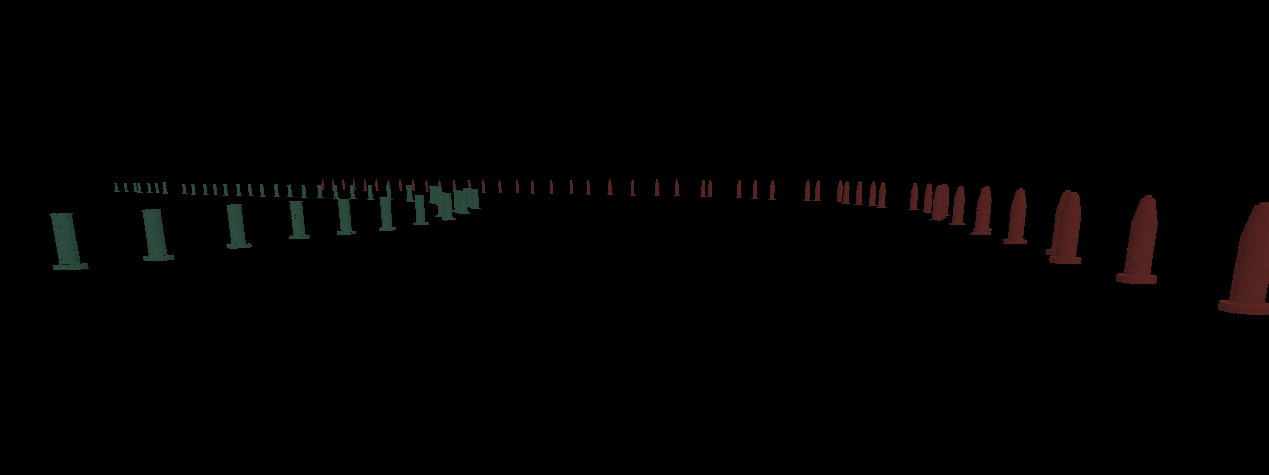
\includegraphics[width=16cm]{img/image_color_segmentation.png}
        \caption{Image after color segmentation}
        \label{fig:color-segmented-image}
    \end{figure}
    
    \item{Resizing}
    
    Images are downscaled from the original 1280x720 resolution to 80x64. It significantly accelerates the training process while keeping all the valuable information.
    
    \item \textbf{Normalization}

    Pixel values are normalized to $[0, 1]$ again for boosting neural network performance, CNN in particular.
    
    \item \textbf{Image stacking}
    
    The last 5 camera images are concatenated into a tensor with dimensions $(64, 80, 3 \times 5)$. The numbers represent height, width, number of channels and sequence length respectively. This approach creates a time series containing enriched information that results in better policy networks compared to a single image. Same method was used in preprocessing stage by \emph{Google Deep Mind} in a state-of-the-art DQN exceeding human-level performance in Atari2600 games \cite{DQNAtari}.
\end{enumerate}

Consequently, after all preprocessing steps have been performed, the observation space is a $3^{rd}$ order $(64 \times 80 \times 15)$ tensor. Values are within $[0, 1]$ range.

\subsubsection*{Reward}
\label{sub2:reward}

There have been various reward systems tested. At first the agent had been rewarded with small value $R_a(s, s')$ for every step that got it closer to the desired point $(x_d, y_d)$ and punished with $-R_a(s, s')$ otherwise. If it managed to reach $(x_d, y_d)$ it was additionally rewarded with much greater \textbf{done reward} $40R_a(s, s')$ and punished with $-40R_a(s, s')$. Although the second reward is undoubtedly necessary to allow the reinforcement network distinguish between successful and unsuccessful episode, the small partial reward was confusing. There were parts of the track which forced the boat to float against the "current". That is in order not to leave the track the agent had to acquire negative rewards throughout several episodes, which was breaking the learning process at some point eventually.

The new approach replaced partial step reward with checkpoint reward. Pairs of corresponding buoys are stored in a LIFO\footnote{Last in first out} list. The agent crosses the checkpoint when both \ref{eq:5.1} \& \ref{eq:5.2} are satisfied and is moving towards desired position. When it occurs, the pair of buoys is popped out from list to prevent the boat from gaining multiple rewards for crossing the same checkpoint. Altogether, the maximum reward equals 

\begin{equation}
R_{max} = N \cdot R_a(s, s') + 40R_a(s, s')
\end{equation}

where $N$ is number of checkpoints.

Such strategy for reward distribution turned out to be effective despite its simplicity.

\section{Deep Reinforcement Network Architectures}
\label{sec:dnn-architectures}

There has been four deep neural network architecture evaluated, all of which base on a DQN described more in depth in section \ref{sec:deep-q-learn}. Each consecutive one was expected to present better performance, because every architecture except the core Deep Q-Network is only an extension which addresses some of know issues of the predecessor. The goal was to compare each network's performance in the same simulation scenario, for an exact set of hyperparameters derived from empirical trials. No grid search was performed owing to high computational cost. The results of such comparison are presented in the following chapter.

\begin{table}
    \centering
    \begin{tabular}{|c c|}
        \hline
        \multicolumn{2}{|c|}{Hyperparameters} \\
        \hline
        learning rate (lr) & $1e^{-5}$ \\
        $\gamma$ & $0.99$ \\
        $\epsilon$ & $1.0$ \\
        $\epsilon$ decrease & $5e^{-5}$ \\
        $\epsilon_{min}$ & $0.01$ \\
        memory size & $1.2e^4$ \\
        batch size & $32$ \\
        replace target network steps & $1000$ \\
        max steps & $1000$ \\
        \hline
    \end{tabular}
    \caption{Hyperparameters used in every architecture}
    \label{tab:hyperparameters}
\end{table}

\subsection{Deep Q-Network}
\label{sub:deep-q-network}

This is the underlying architecture behind every network in the research. It was highly inspired by \emph{Google Deep Mind} research from 2015 \cite{DQNAtari}, which has been already mentioned in the Thesis. Although this DQN has presented outstanding performance in the Atari2600 environment it had been questionable whether same results would be observed in the Gazebo environment. There are considerably more distinct states which differ only slightly from one another. Unlike the Atari game where screens change more dynamically and contain more characteristic features.

Most of the key concepts behind the implementation of Deep Q-Network, such as \emph{temporal difference}, \emph{q-value}, \emph{experience replay}, \emph{markov decision process} or \emph{bellman equation}, have been already discussed in sections \ref{sec:q-learn} and \ref{sec:deep-q-learn}.
The issue with direct implementation of those is that reinforcement learning is known to be unstable or even to diverge when a nonlinear function approximator such as a neural network is used to represent the action-value (Q) function. These instabilities are addressed by experience replay (\ref{sub:experience-replay}) and splitting evaluation and prediction into \textbf{Evaluation Q-Network (Q-eval)} and \textbf{Target Q-Network (Q-Target)}. Whereas the first one is used to update weights using stochastic gradient descent and a loss function, the latter is used to make predictions about the next action. The action-value function $Q(s, a; \theta_i)$ is parameterized, where $\theta_i$ are the weights of the Q-network at iteration $i$. Target network is an exact copy of the evaluation network having parameters $\theta^-_i$ replaced (copied $\theta_i$ from the evaluation network) every $C$ steps and held fixed between individual updates. This approach significantly stabilises learning process.

Experience replay $e_t = (s_t, a_t, R_{at}(s, s'), s_{t+1})$ is stored at each time step $t$ in a buffer $D_t = \{e_{\max\left(1, (t - mem\_size)\right)}, ..., e_t\}$. During learning there are updates applied on uniformly drawn samples of experience $U(D)$ of size $batch\_size$. The update means backpropagating stochastic gradient descent at iteration $i$ using the following loss

\begin{equation}
    L_i(\theta_i) = \sum_{(s, s') \sim U(D)}P_a(s, s')\left(R_a(s, s') + \gamma \max_{a'} Q(s', a'; \theta^-_i) - Q(s, a; \theta_i) \right)^2
\label{eq:deep-q-loss}
\end{equation}

Which is actually a squared, parameterized temporal difference (\ref{sub:temporal-difference-learning}).

\subsubsection*{Model Architecture}
\label{sub2:model architecture}

The architecture used takes as an input state observation (\ref{sub2:observation-space}) and returns predicted Q-values for all possible
actions. The greatest advantage of such solution is that only one forward pass is needed to compute Q-value for every action. The input to the
neural network consist of 5 stacked $64 \times 80$ images. There are three convolutional layers in the network, each proceeded by ReLU
(\ref{sec:activation-function}) and max pool (\ref{sec:conv-pooling}) operations. The convolutional layers use 32, 64, 64 filters of $3 \times 3$
size. The max pool layers use $2 \times 2$ filter reducing the size of input $8$ times to $8 \times 10$. The hidden fully connected layer consist
of 256 linear rectifier units. The output layer is a fully-connected linear layer with number of outputs representing number of actions, in our
case $8$.

\begin{figure}[h]
    \centering
    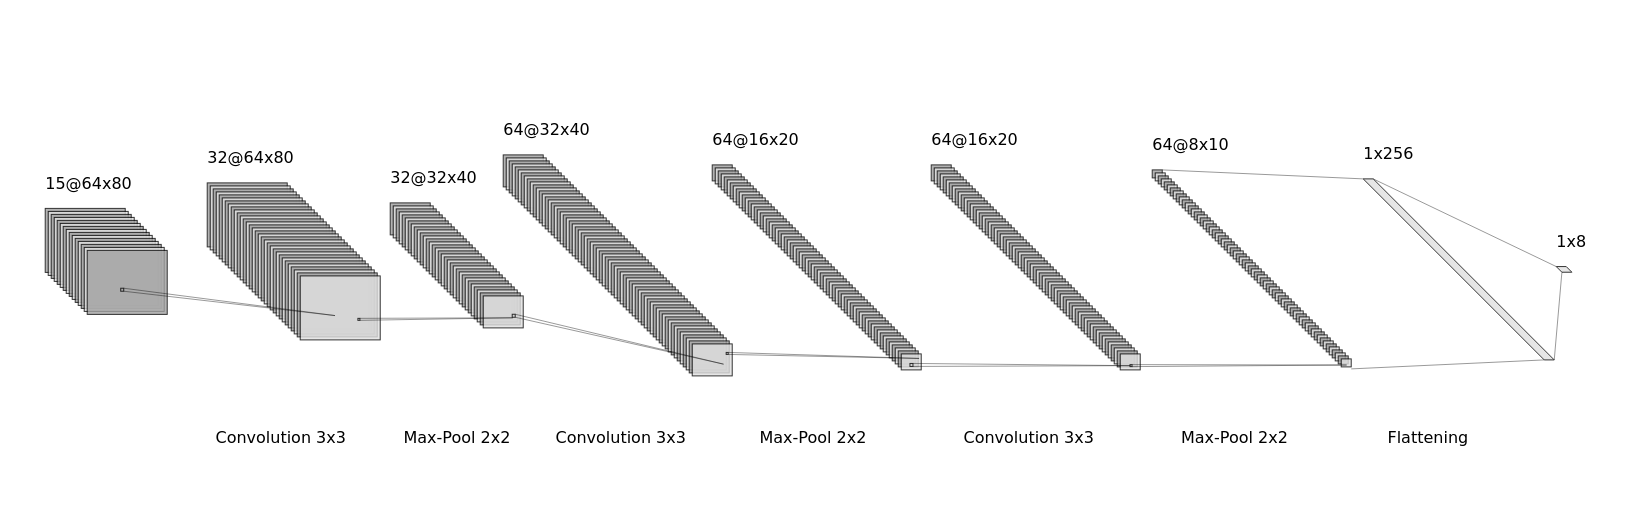
\includegraphics[width=16cm]{img/model-architecture.png}
    \caption{DQN network used in the vision system}
    \label{fig:dqn-network}
\end{figure}

\subsubsection*{Algorithm}
\label{sub2:dqn-algorithm}

The algorithm steps are nearly identical to the Q-learning (\ref{sec:q-learn}) with the exception that nonlinear approximator is used instead of a
linear one. Therefore optimal action-value function is estimated as $Q(s, a; \theta) \approx Q^*(s, a)$. The neural network approximator with
weights $\theta$ is referred as Deep Q-network. It is trained by adjusting weights $\theta_i$ at step $i$ to reduce loss function where target
values $y = R_a(s, s') + \gamma \max_{a'}Q^*(s', a')$ are replaced by approximate target values $y = R_a(s, s') + \gamma \max_{a'}Q(s',
a';\theta^-_i)$ using weights $\theta^-_i$ from some previous step.

This Deep Q-learning algorithm is also an model-free and off-policy algorithm, just as a regular Q-learning. The agent follows a policy $\pi(s)$
ensuring adequate exploration-exploitation balance while learning about the greedy policy $\pi^*(s) = arg\max_{a'}Q(s, a'; \theta)$.

\subsubsection*{Training algorithm for Deep Q-Networks}
\label{sub2:training-algo-for-deep-q-net}

The full algorithm is presented in listing below. It uses already explained concepts as experience replay or two networks - evaluation $Q$ and
target $\hat{Q}$ to make it possible to train a large ANN without diverging. In a standard Q-learning approach every update that increases $Q(s,
a)$ also increases $Q(s', a)$ for all $a$ subsequently resulting in an increase of the target $y$. This may lead to undesired oscillations or
divergence of the policy. Using two networks addresses this issue. Additionally, clipping the error from loss function \ref{eq:deep-q-loss}
$\left(R_a(s, s') + \gamma \max_{a'} Q(s', a'; \theta^-_i) - Q(s, a; \theta_i) \right)$ to $[-1, 1]$ also increased the stability of the algorithm.

The entire algorithm was written in \emph{Python} 3.9.7 using \emph{pytorch} 1.9.1 library. An image preprocessing part was held in
\emp{opencv-python} 4.5.3.56. Source code with all dependencies can be found at \emph{github
repository}\footnote{\url{https://github.com/A-NGJ/bachelor_thesis}}.

\begin{lstlisting}[language=Python, caption={Main algorithm loop}]
1  agent = Agent(**hyperparameters)
2  agent.initialize_memory(mem_size)
3  # initialize evaluation network with random weights
4  agent.initialize_q_eval()
5  # initialize target network with identical weights to q_eval
6  agent.initialize_q_target()
7  for i in range(epochs):
8      done = False
9      observation = env.reset() # start with fresh environment
10     game_steps = 0 # steps per epoch accumulator
11     steps = 0 # overall steps accumulator
12        
13     while not done:
14         if random(min=0, max=1) > epsilon:
15             # feed forward observation through DQN to get q-values for each action
16             # choose the action which maximises Q
17             action = argmax(q_eval.forward(observation))
18         else:
19             # chose random action from action space
20             action = random_choice(action_space)
21            
22         # execute action in a simulator
23         next_observation, reward, done = env.step(action)
24         # store transition in a memory
25         agent.store_transition(observation, action, reward,
26                                next_observation, done)
27         # start learning only after it was filled with samples
28         if memory.is_filled:
29             if steps % replace_frequency:
30                 q_target.load_parameters_from(q_eval)
31         # Sample minibatch of size batch_size from the memory
32         observations, actions, rewards, next_observations, dones =\\
33             sample_memory(size=batch_size)
34         # Get q-values for actions predicted by both evalueation and target network
35         q_pred = q_eval.forward(observations)
36         q_next = q_target.forward(next_observations)
37         # if episode terminates after an action, target value is equal only to reward
38         q_next[dones] = 0.0
39         # Plural names are used because operations are performed 
40         # on the entire minibatch
41         q_target = rewards * gamma*q_next
42         # Perform a gradient descent, MSE loss is used
43         loss = q_eval.loss(q_target, q_pred)
44         # Clip error between -1 and 1
45         loss.clip(-1, 1)
46         q_eval.backpropagate(loss)
47         decrement_epsilon(eps_dec)
48              
49         observation = next_observation
50         game_steps += 1
51         steps += 1
52         # Terminate an episode if maximum number of steps has been reached
53         if game_steps > max_steps:
54             break
\end{lstlisting}

\subsection{Double Deep Q-Network}
\label{sub:double-deep-q-network}

Although Deep Q-Network is capable of finding good approximation of optimal policy, it is not flawless. As \emph{Hado van Hasselt}, \emph{Arthur Guez} and \emph{David Silver} \cite{DBLP:journals/corr/HasseltGS15} show that DQN sometimes substantially overestimates the values of the actions. In a DQN evaluation

\begin{equation}
    y_i = R_a(s, s') + \gamma \max_{a'}Q(s', a'; \theta^-_i)
\end{equation}

the \emp{max} operator uses equal values both to select and to evaluate an action. This leads to overoptimistic estimations of values. In order to address that issue action selection can be separated from action evaluation. This is the main concept behind \textbf{Double Deep Q-learning}. Slight change which leads to significant improvement in preventing the value overestimation. Luckily, DQN architecture provides natural candidate for a action-value function which would replace the \emph{max} operator. The evaluation network is used, as the name suggests, to evaluate the greedy policy whereas a target network estimates its value.

\begin{equation}
    y_i = R_a(s, s') + \gamma \hat{Q}(s', arg\max_{a'}Q(s', a'; \theta_i); \theta^-_i)
\end{equation}

That is it! A performance boost with perhaps minimal possible change to DQN. The rest of algorithm stays intact, so the only change we need to introduce is in lines 35 - 41:

\begin{lstlisting}[language=Python, caption={Double Deep Q-learning modification}]
35  q_pred = q_eval.forward(observations)
36  q_next = q_target.forward(next_observations)
37  q_eval = q_eval.forward(next_obsevations)
38  q_next[dones] = 0.0
39  q_target = rewards + gamma*q_next[argmax(q_eval)]
\end{lstlisting}

\subsection{Dueling Deep Q-Network}
\label{sub:dueling-deep-q-network}

Dueling network architecture was first proposed by \emph{Ziyu Wang  et al.} \cite{DBLP:journals/corr/WangFL15}. It was a direct approach to 
improve model-free RL models. The underlying idea is to separate the representation of state values $V(s)$ and state dependent action 
advantages $A(s, a)$. Unlike DQN or DDQN it consist of two streams that represent the value and adavantage functions, as shown below.

\begin{figure}[h]
    \centering
    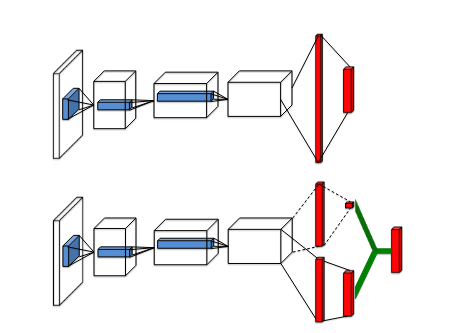
\includegraphics[width=10cm]{img/dueling_vs_single_qn.png}
    \caption{Single stream Deep Q-Network (top) and Dueling Deep Q-Network (bottom). Source \cite{DBLP:journals/corr/WangFL15}}
    \label{fig:single-vs-dueling-q-network}
\end{figure}

The \textbf{advantage function} is defined as

\begin{equation}
    A(s, a) = Q(s, a) - V(s)
\label{eq:advantage}
\end{equation}

It measures how good is actually every action $a$ while being in state $s$. If we think of $Q(s, a)$ as a quality of each action that can be
taken in a particular state and $V(s)$ as a actual value of given state, the difference is a pure action importance. If the action does not 
change the state substantially it means that action is rather negligible. On the other hand, if the difference is high, the action must be
influential. Intuitively it makes absolute sense. Taking as an example our simulation, in most of states it does not matter whether the
agents floats slightly left or right, as long as it is not at the track edge. Note that for the greedy policy $a^* = \pi^*(s) =
arg\max_aQ(s, a)$, it follows that $Q^*(s, a) = V^*(s, a^*)$ therefore $A(s, a^*) = 0$.

The Dueling DQN architecture is identical to DQN until the point of fully connected layer, where instead of single sequence of fully
connected layers, there are used two. The separate streams are capable of providing estimates of the value and advantage functions.
Subsequently these streams are combined to output a set of Q-values, one for each action $a \in A$\footnote{In this section bare $A$
represents action space, as it did through the entire Thesis, whereas $A(s, a)$ represents advantage function.}
The state value approximation network can be expressed as $V(s; \theta, \beta)$ and advantage approximation network as $A(s, a; \theta,
\alpha)$. Where $\theta$ are the parameters of convolutional layers, $\beta$ denotes the weights of fully connected value network and
$\alpha$ analogously for the advantage network.

Constructing the aggregate module which is the approximation for Q function is not that straightforward though. Using directly the advantage definition (\ref{eq:advantage})

\begin{equation}
    Q(s, a; \theta, \alpha, \beta) = V(s; \theta, \beta) + A(s, a; \theta, \alpha)
\end{equation}

leads to the identifiability problem. That is, it is impossible to recover $V(s)$ and $A(s, a)$ from the given $Q$. In order to address
that, the advantage function estimator can be forced to have zero advantage at the chosen action.

\begin{equation}
    Q(s, a; \theta, \alpha, \beta) = V(s; \theta, \beta) + \left(A(s, a; \theta, \alpha) - \frac{1}{|A|} \sum_a A(s, a; \theta, \alpha)\right)
\end{equation}

Now every time the advantages change as fast as the mean the above equation has the form of $Q(s, a; \theta, \alpha, \beta) = V(s; \theta,
\beta)$. Therefore it is clear which stream provides estimate of the value function and which the estimate of the advantage function.

In order to implement Dueling DQN architecture, lines 35-36 again have to be modified. This change literally replaces single fully connected layer stream with dual, remaining parts stay intact.

\begin{lstlisting}[language=Python, caption={Dueling Deep Q-learning modification}]
35  V_s, A_s = q_eval.forward(observations)
36  V_s_next, A_s_next = q_target.forward(next_observations)
37  q_pred = V_s + (A_s - mean(A_s))
38  q_next = V_s_next + (A_s_next - mean(A_s_next))
\end{lstlisting}

Where \emph{V\_s} is the output of Value layer having only one output and \emph{A\_s} is the output of advantage layer having $N_{outputs}= |A|$.

\subsection{Dueling Double Deep Q-Network}
\label{sub:dueling-double-deep-q-network}

Having discussed Double DQN and Dueling DQN architectures one may notice that it is possible to combine them into a new robust Dueling
Double Deep Q-Network architecture\footnote{DDDQN in short or D3QN, which gives reader the flexibility to decide whether "Double" stands
behind or in front of "Dueling".}. Since Dueling DQN preserves the Q-values output, only modifying the way they are estimated, it is
perfectly feasible to use these Q-values in action selection and action evaluation as it is performed in Double DQN. Such combination
results in the following target value

\begin{equation}
    y_i = R_a(s, s') + \gamma \hat{Q}(s', arg\max_{a'}Q(s', a'; \theta_i, \alpha_i, \beta_i); \theta^-_i, \alpha^-_i, \beta^-_i)
\label{eq:dueling-double-dqn-target-value}
\end{equation}

Where $\alpha^-_i$ and $\beta^-_i$ are respectively weights of advantage and value streams from some previous step.

The modification in source code, again begins at line 35 and requires little effort.

\begin{lstlisting}[language=Python, caption={Dueling Double Deep Q-learning modification}]
35  V_s, A_s = q_eval.forward(observations)
36  V_s_next, A_s_next = q_target.forward(next_observations)
37  V_s_eval, A_s_eval = q_eval.forward(next_observations)
38    
39  q_pred = V_s + (A_s - mean(A_s))
40  q_next = V_s_next + (A_s_next - mean(A_s_next))
41  q_eval = V_s_eval + (A_s_eval - meand(A_s_eval))
42    
43  q_target = rewards + gamma*q_next[argmax(q_eval)]
\end{lstlisting}

This is the most sophisticated modification of the DQN architecture and even so it keeps most of the code unchanged. It can be said that
the subsequent DQN network architectures (\ref{sub:double-deep-q-network}, \ref{sub:dueling-deep-q-network},
\ref{sub:dueling-double-deep-q-network}) follow object oriented programming principles. They inherit from well defined base and add or
overwrite only necessary functionalities.

\subsection{Training details}
\label{sub:training-details}

The training was performed in a fixed simulation environment described in \ref{sec:simulation-env}. Hyperparameters were set to values from
table \ref{tab:hyperparameters}. They were identical for every network architecture. Each network architecture described above has been
trained from scratch for 700 epochs keeping track of score and average Q-value along single episode. These indicators were further crucial
in model evaluation and comparison. Due to hardware limitations it was impossible to train a model for a longer period even though it was
clear that longer training would have resulted in a better outcome. The entire training lasted 8-12h and was susceptible to unexpected
system errors, because the simulation environment was unstable when it was running for the extended time. Therefore tuning hyperparameters
took considerable amount of time and for some fixtures the evaluation had to be rerun. It is unclear whether the hyperparameters proposed
in the section are optimal, yet these are the ones for which the agent managed to acquire highest score. A grid search was not performed
owing to high computational cost and time limitations. The final parameters base on a empirical results and architectures proposed in
(\cite{DQNAtari}, \cite{2020DuckieTown}, \cite{DBLP:journals/corr/HasseltGS15}, \cite{DBLP:journals/corr/WangFL15}).

In the experiments there was used RMSProp optimization algorithm and in the entire training there were used on average 80000 frames. The setup used minimal amount of prior knowledge: the input data consisted only of visual images retrieved from boat's front cameras and number of actions. Everything that the agent learned was learned from exploration and experience.